\chapter{Cost Modeling for an\\EGS Power Plant Expansion}\label{ch4:cm_prep}

The second of the two research questions presented in Chapter \ref{ch1:intro} addressed the topic of risk in geothermal development and production. As discussed in Chapter \ref{ch2:background}, production planning generally includes economic analysis of the subsurface conditions, development plan, and power plant concept projected over the anticipated lifespan of a field. This chapter describes a methodology for modeling the value of an EGS power generation project, applied to the Lightning Dock KGRA in Southwestern New Mexico. The method combines uncertainties and variable operational strategies to mitigate risk in geothermal production.

\section{EGS Expansion Concept}\label{ch4:cm_concept}
\subsection{Lightning Dock EGS}\label{ch4:lightning_dock_egs}
Lightning Dock is presently the only commercial power plant operating in the state of New Mexico (see Section \ref{ch2:lightning_dock}). The net generating capacity after its first phase of development was 4 MW in 2013. An expected second-phase upgrade to 10 MW never came to fruition. Instead, the facility underwent a significant refit in 2018, resulting in a net capacity of 11.2 MW generated entirely from hydrothermal brine production \citep{bonafin_repowering_2019}.

DOE-funded efforts to characterize the geothermal resources of the Animas Valley --- where Lightning Dock is located --- revealed the presence of two different thermal reservoirs: the hydrothermal resource targeted by Lightning Dock where deep geothermal fluids ascend along the Animas Valley Fault complex to $\approx$365-1000 m depth, and a secondary interval at $\approx$900-1200 m depth that requires permeability enhancement for production \citep{schochet_development_2001}. The Horquilla limestone formation defines the second reservoir, estimated to span a minimum volume of 6 cubic km based on conservative figures. By one proprietary study completed in 2001 for Ormat International, the Horquilla has a most-likely production potential of 9.3 MW, and an 88\% probability of exceeding 6 MW \citep{schochet_development_2001}.

\citet{schochet_development_2001} proposed the construction of a 6 MW hybrid power plant combining hydrothermal and EGS-sourced power generation a decade before operations commenced at Lightning Dock. In their development plan, they noted several benefits of pursuing EGS in this location:
\begin{itemize}[itemsep=2pt]\label{ch4:ld_egs_support}
    \item Relatively shallow resource equates to lower drilling costs
    \item EGS water requirements attainable from paired hydrothermal operations
    \item Low/no assessed environmental impact from geothermal operations
    \item Direct access to in-place transmission lines  
    \item Opportunity for direct electricity sales to local users
    \item Purchase agreements with regional utilities incentivized by NM legislation
\end{itemize}

As suggested by this list, conditions at Lightning Dock offer a nearly ideal test case for an EGS proof of concept on a manageable scale. In addition, land utilization in the area is historically agricultural with few residences, so risk is low for adverse impact on an existing population. And the use of binary cycle generation as proposed by \citet{schochet_development_2001} supports power production with zero greenhouse gas emissions.  

In this thesis, the \citeauthor{schochet_development_2001} concept is revisited with the existing geothermal production at Lightning Dock kept in mind; rather than building a new hybrid facility, the revised concept involves targeting the deeper reservoir as a NF-EGS development that ties back to the current Lightning Dock facility. Stepping out from the hydrothermal zone in proximity to the Animas Valley Fault complex, thermal conditions settle to a high background geothermal gradient between $\approx$ 80-120 K/km based on boreholes TG 56-14 and TG 12-7 \citep{cunniff_final_2003} --- high enough to support geothermal capture. These conditions make for an interesting case study on risk mitigation options for EGS production planning founded on a NF-EGS concept that was already proven at The Geysers \citep{pan_establishment_2019}.

Public records regarding power generation at Lightning Dock provide some guidance on the appropriate size of such an EGS expansion. After its original phase 1 development, the plant produced 4 MW. An additional 6 MW was slated for phase 2, but re-powering of the plant actually added 7 MW to the capacity after several years of development stasis \citep{think_geoenergy_turboden_2020}. \citeauthor{schochet_development_2001} originally proposed a 6 MW hybrid plant for the site, but they also noted 6 MW was likely understating the full reservoir potential of the Horquilla alone (\citeyear{schochet_development_2001}). In consideration of the step-wise trajectory of plant improvements and the assessment of available thermal resources, this case study targets 5 MW as an expansion goal. 

\subsection{New Mexico Electricity Demand}\label{ch4:nm_rps}
Pursuing the expansion of a power plant requires sufficient demand to ensure total revenue offsets project expenses. Fortunately, New Mexico regulations support further development of geothermal power production in the state. Specifically, the Energy Transition Act signed in 2019 updated the New Mexico \acrlong{rps} (\acrshort{rps}) to go zero-carbon by 2050, with milestone targets along the way \citep{lillian_new_2019}. The RPS dates back to the Renewable Energy Act passed in 2004 and comes with several carve-outs, including a 30\% requirement for wind energy, 20\% for solar, and 5\% for other renewables like geothermal \citep{dsire_dsire_2021}. Public Service Company of New Mexico (PNM) is the state’s largest energy provider and services the Lordsburg area where Lightning Dock is located. PNM and Cyrq Energy currently share a 20-year \acrlong{ppa} (\acrshort{ppa}) for electricity generated at Lightning Dock. The PPA has gone through amendments over time to update both the wattage supplied to PNM and the pricing structure per MWh \citep[e.g.,][]{pnm_public_2014,stanfield_new_2017}. This indicates a willingness to revisit a PPA if conditions change, which is an important aspect to consider when modeling project financials.

In addition to the RPS requirement for a diversified portfolio, coal power plants across the state face mandated shut-downs as a consequence off the Energy Transition Act. Coal currently supplies a large fraction ($\approx$ 37\%) of in-state electricity generation \citep{eia_new_2021} and nearly $20\%$ of consumed energy in New Mexico (Figure \ref{fig:nm_energy_consumption}). The supply gap introduced as coal-based production drops to zero could more than compensate for a 5 MW addition of no-emissions energy to the New Mexico grid.

\begin{figure}[!htp]
\centering
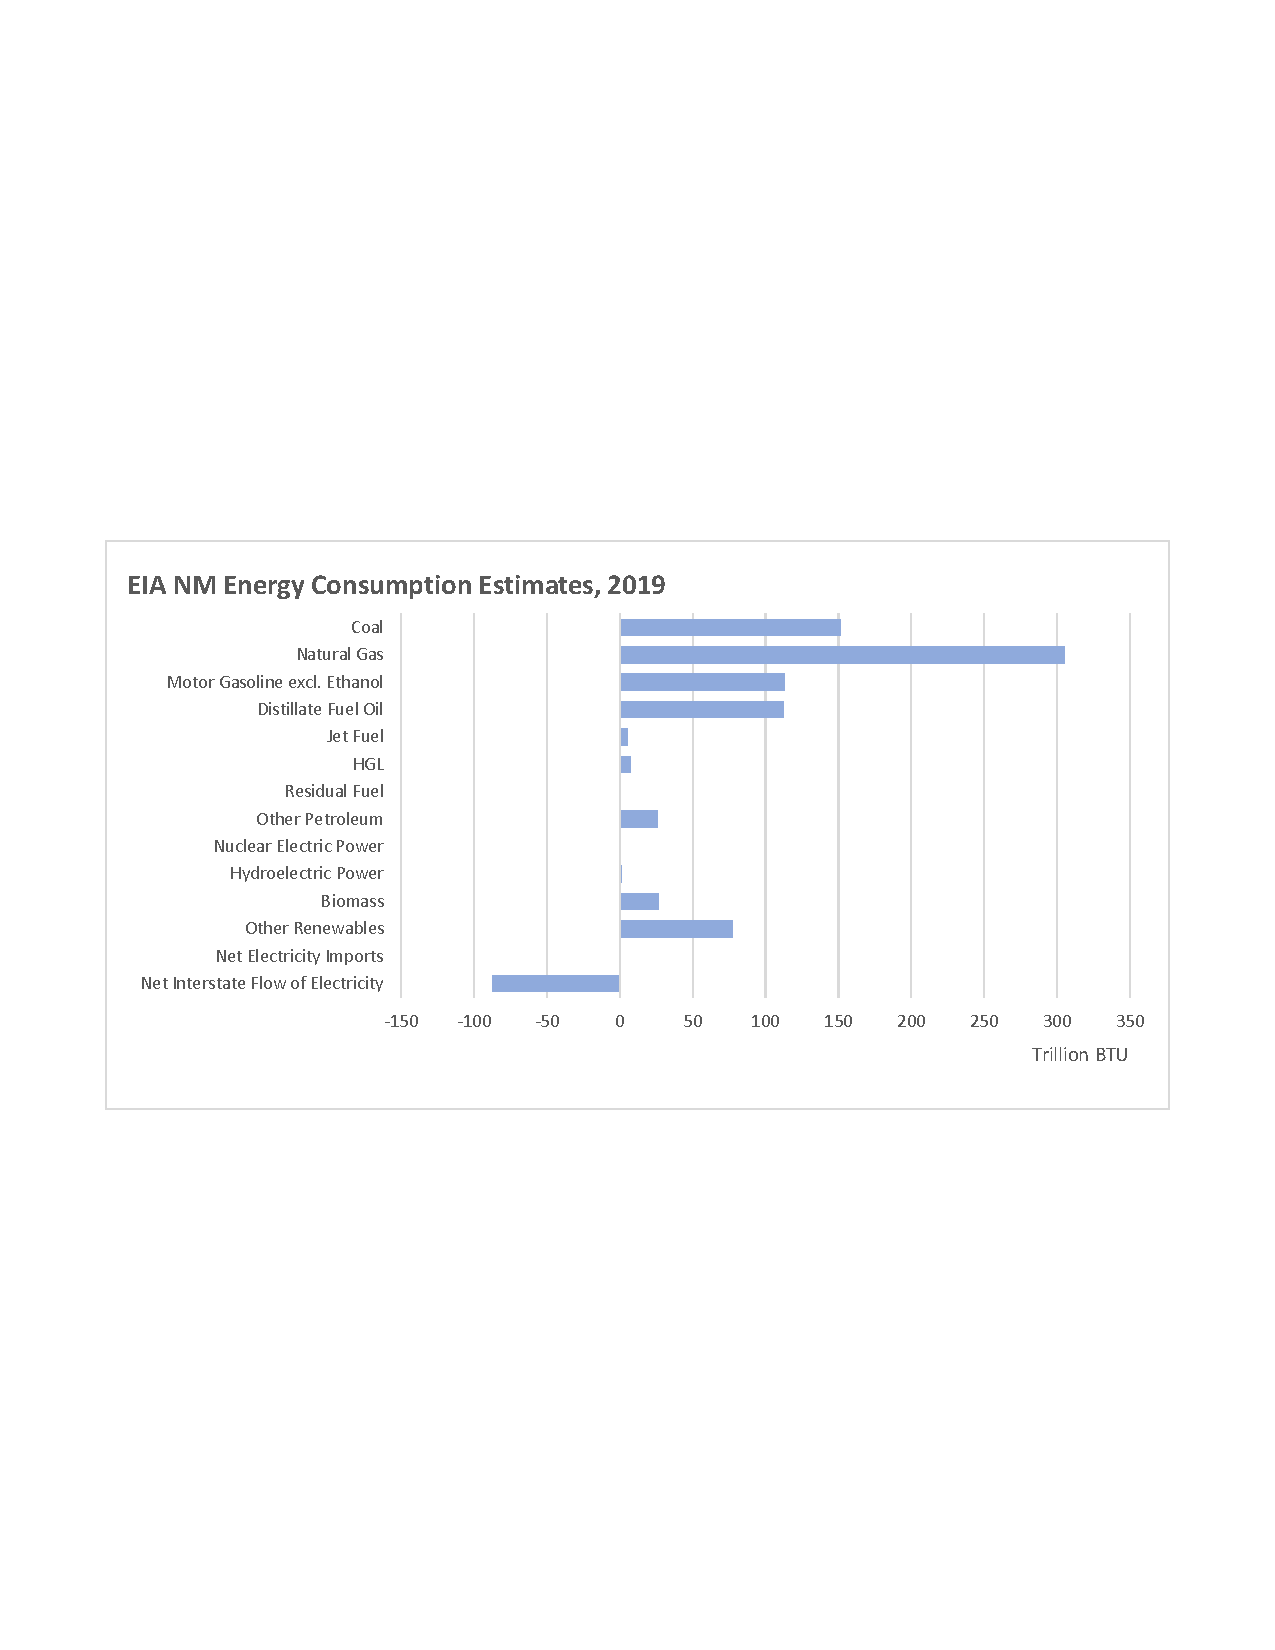
\includegraphics[width=\textwidth]{templates/images/Figure-EIA_NM_Energy_Consumption.pdf}
\caption[New Mexico energy consumption]{Energy consumption by source for New Mexico. Adapted from data and graphics reported by the EIA \protect\citep{eia_new_2021}.}
\label{fig:nm_energy_consumption}
\end{figure}

\subsection{Modular Geothermal}\label{ch4:modular_geothermal}
Limiting the expansion to a single 5 MW facility represents one design alternative, but others exist as well. One flexible option uses modular technology that recently captured the attention of high-stakes investors across the world \citep{shieber_bill_2019}. Climeon has engineered a compact binary cycle unit capable of 150 kW of generated electricity using inlet fluid temperatures rated up to 120℃ and flow rates of up to 35 kg/s \citep{climeon_climeon_2021-1}. These units can be combined into a larger deployable ``Power Block'' for 1050 kW of electric capacity \citep{winther_power_2018} (Figure \ref{fig:climeon_powerblock}). Using this technology, power plants can now be treated like multi-unit assemblages, installed all at once or over an extended period of time based on operator needs \citep{climeon_why_2018}.

\begin{figure}[!htp]
\centering
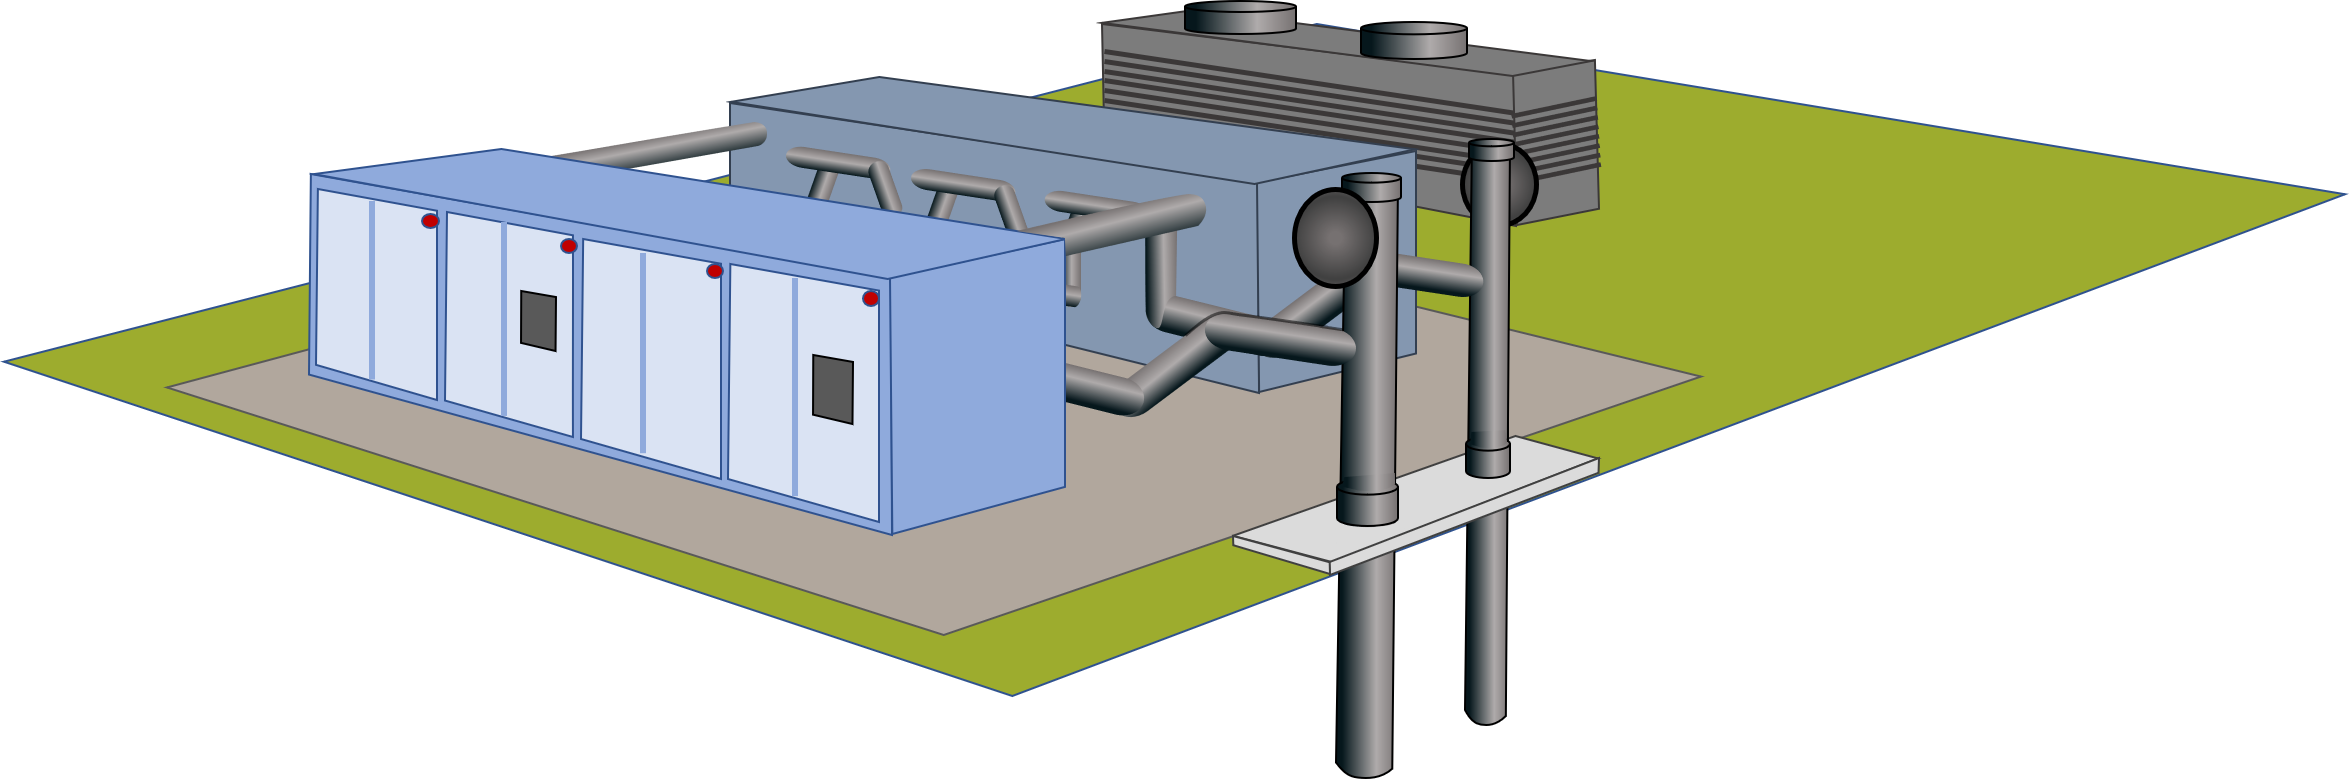
\includegraphics[width=\textwidth]{templates/images/Figure-Climeon-PowerBlock.png}
\caption[Modular power plant schematic]{Modular binary cycle power plant concept, adapted from Climeon PowerBlock schematic diagram \protect\citep{climeon_climeon_2021-1}. Each block consists of seven active units chained together for $\approx$1 MW of generating capacity.}
\label{fig:climeon_powerblock}
\end{figure}

\subsection{Flexible Cost Models}\label{ch4:flex_models}
As discussed in Section \ref{ch2:cost_models}, cost models can provide insights into the potential value gained or lost by a proposed facility before construction even begins. Well-established geothermal cost models like GETEM \citep{entingh_volume_2006} present a highly parameterized but deterministic view of cost and investment opportunity given a defined geothermal resource and development concept. Other models may apply different assumptions or mathematical treatments for various facets of the system, however they uniformly offer a single-track aspect to how the project unfolds over its lifecycle. Users can test ideas, but the solution space remains under-explored due to implicit assumptions of variable trends or static behaviors for a highly-dynamic system.

In the cost model outlined below, the economic analysis incorporates uncertainty by replacing single value estimates with distributions for model variables. This enables the model to produce a representative range of possible outcomes when simulated many times over. In addition, the model flexibly adapts by executing design options, where model updates triggered by changing conditions allow the system to realize upside potential or characterize the extent of downside risk. Designs need not be static, and flexibilities can greatly increase the expected value of a project by exploring execution strategies otherwise missed by more traditional modeling approaches \citep[Chapter 6]{de_neufville_flexibility_2011}.

\section{Static Cost Model}\label{ch4:cm_structure}
Geothermal cost models typically report Levelized Cost of Electricity (LCOE) for simple comparison with other renewable energy sources. However, LCOE is standardized to represent the total lifetime costs incurred by a power plant normalized by the total power generation from start-up to plant decommissioning. LCOE is thus not well-suited for communicating projected gains or losses under different plant designs or scenarios, which are the focus of this analysis. Instead, the model described here relies on \acrlong{npv} (\acrshort{npv}), a simple measure of project worth that accounts for the time value of money by applying a single interest rate, the discount rate, for both borrowing and deposits \citep[p.\ 195-215]{de_neufville_flexibility_2011}. Here, ``present value'' refers to a 2020 cost basis. For power generation over a 30-year lifespan -- the default for geothermal models like GETEM \citep{entingh_volume_2006} -- this basis takes the model out to 2050, a common benchmark year for future projections. 

\subsection{NPV Model}\label{ch4:cm_npv}
Following the general outline for geothermal cost modeling from previous work \citep[e.g.,][]{augustine_hydrothermal_2009, beckers_introducing_2013,tester_future_2006}, this thesis considers revenue (R), operating \& maintenance costs (\acrshort{opex} or OM), and capital expenditures (\acrshort{capex} or C) as the primary components defining annual cash flow (see Equation \ref{eq:cm_components}). Capital expenses can be further decomposed into five  sub-components associated with exploration, drilling, reservoir stimulation, fluid distribution, and power plant costs. Likewise, operating expenses subdivide into subsidiary costs for the power plant, wells, and water management.
\begin{equation}
    \label{eq:cm_components}
    \begin{aligned}
    NPV &= \sum_{t=1}^{T}D_t \cdot \left( R_t - C_t - OM_t \right)\\
    \text{where:}\\
    C_t &= \left[C_{expl} + C_{dc} + C_{stim} + C_{dist} + C_{pp}\right]_t\\
    OM_t &= \left[OM_{pp} + OM_{well} + OM_{water}\right]_t
    \end{aligned}
\end{equation}
Revenue and expenses are treated on an annual basis, meaning shorter-term fluctuations like price and production seasonality are not explicitly modeled. $D_t$ in Equation \ref{eq:cm_components} defines the time-based conversion factor between cash flow for a specific year and discounted cash flow for the basis year (see Equation \ref{eq:discount_rate}).

\subsubsection{Revenue}\label{ch4:cm_rev}
Annual revenue calculations rely on an estimate of power production within a year ($W$) and the power purchase agreement pricing ($p_{PPA}$) for that electricity \citep{entingh_volume_2006}. 
\begin{equation}
    \label{eq:cm_rev}
    R = W \cdot p_{PPA} = (b_e \cdot \dot{m}) \cdot p_{PPA}
\end{equation}
Brine effectiveness ($b_e$) describes the electricity output per unit flow of produced brine ($\dot{m}$) and depends on the production temperature of the brine. The GETEM model uses an empirically-defined relationship with brine temperature ($^\circ$C) to determine brine effectiveness (w-hr/kg) \citep[p.\ 62]{entingh_volume_2006}:
\begin{equation}
\begin{aligned}
    \label{eq:brine_eff}
    b_e &= C_0 + C_1 \cdot T_{prod} + C_2 \cdot T_{prod}^2 + C_3 \cdot T_{prod}^3 + C_4 \cdot T_{prod}^4 \\
    &\quad C_0 = 9.41376 \\
    &\quad C_1 = -0.182542 \\
    &\quad C_2 = 0.0001765735 \\
    &\quad C_3 = 0.000012204486 \\
    &\quad C_4 = -0.0000000335559
\end{aligned}
\end{equation}

In the GETEM interface, users choose to either determine electricity output for a specified input temperature and flow rate, or alternatively, derive the flow rate required to meet a pre-determined power sales capacity for the same fluid temperature \citep{entingh_volume_2006}. Since the Climeon analog has a known net capacity of 150 kW per unit or 1.05 MW for each Power Block \citep{climeon_climeon_2021-1}, and standard flow rates are provided in models like GETEM, both options are explored in Chapter \ref{ch6:cm_results}.

\subsubsection{Exploration Capital Expenses}\label{ch4:cm_capex_expl}
Costs for exploration activities are estimated by the same method defined for the 2012 GETEM model (Equation \ref{eq:cm_capex_expl}) \citep{eere_getem_2012}. 

\begin{equation}
\label{eq:cm_capex_expl}
    C_{expl} = PPI \cdot \left[ 1.12 \cdot (\$1\text{M} + 0.6\cdot C_{dc}) \right]
\end{equation}

This relationship assumes slim hole (3-6" diameter) drilling for exploration at a 60\% discounted cost compared to standard-sized ($\geq$ 8.5" diameter) geothermal wells \citep{eere_getem_2012}. The constant \$1M term accounts for pre-drilling costs, including field work, geophysical surveys of field structure, and interpretation of results \citep{eere_getem_2012}. Technical and office support is covered by an additional 12\% applied to the estimate \citep{eere_getem_2012}. Total exploration costs are converted to a 2020 cost basis using the \acrlong{ppi} (\acrshort{ppi}) for electric power generation from the U.S. Bureau of Labor and Statistics \citep{us_bls_ppi_2021}.

\subsubsection{Drilling Capital Expenses} \label{ch4:cm_capex_dc}
Geothermal drilling costs differ from traditional oil \& gas wells due to differences in hole diameter, thermal and geochemical conditions, and the strength and abrasiveness of the target formations \citep{lowry_geovision_2017}. Here, drilling capital expenditures rely on a cost curve described by \citet[Eq. 4,\ ][]{beckers_introducing_2013}.

\begin{equation}
\label{eq:cm_cdc}
    C_{dc} = PPI \cdot \left[ 1.65 \cdot 10^{-5} \cdot \text{MD}^{1.607} \right]
\end{equation}
where $C_{dc}$ is measured in \$M and MD refers to well measured depth in meters. Each power plant module will require an injector-producer pair, so this represents one-half of the drilling cost per module. Drilling costs are converted to a 2020 cost basis using the PPI for electric power generation \citep{us_bls_ppi_2021}. 

Note that Equation \ref{eq:cm_cdc} was derived for well depths of 1600-9000 m. Assuming an average geothermal gradient of 100 K/km (Table \ref{tab:cm_resource_params}), the wells considered for this study could extend slightly shallower than this range, so this should be viewed as a minimum drilling estimate. The probabilistic model considered later in this study includes variability in both geothermal gradient and drilling costs for a more comprehensive treatment of both variables.

\subsubsection{Simulation Capital Expenses}\label{ch4:cm_stim}
EGS at Lightning Dock requires stimulation of the Horquilla reservoir to create fluid pathways for thermal extraction. The stimulation cost estimate used in this study comes from the recent GeoVision analysis \citep{lowry_geovision_2017}:

\begin{equation}
\label{eq:cm_capex_stim}
    C_{stim} = \$1,250,000
\end{equation}

Since this represents a recent ballpark estimate, no cost basis conversion was applied in the model. In fact, the value in Equation \ref{eq:cm_capex_stim} may be high since it includes the cost of water, which may not be a factor at Lightning Dock with the availability of hydrothermal brine from adjacent power plant operations. The model assumes stimulation is only performed for the injection well in each injector-producer pair, so this represents a \textit{per module} value.

\subsubsection{Distribution Capital Expenses}\label{ch4:cm_capex_dist}
Fluid distribution costs include the entire surface piping system between the wells and power plant modules. This study uses the same estimate included in the GEOPHIRES model \citep{beckers_introducing_2013}.

\begin{equation}
\label{eq:cm_dist}
    C_{dist} = PPI \cdot \left[ \$50,000 \cdot q_{in} \right]
\end{equation}
where $q_{in}$ is the heat input from the produced brine and $PPI$ converts this 2012 value to a 2020 cost basis. 

The 2nd Law efficiency or thermodynamic efficiency ($\eta$) governs how much heat from the input fluid can be converted to work. \citeauthor{beckers_low-temperature_2016} provides an estimate for sub-critical ORC power plant thermodynamic efficiency as follows (\citeyear[p.\ 39-41]{beckers_low-temperature_2016}):

\begin{equation}
\begin{aligned}
    \label{eq:2ndlaw_eff}
    \eta &= K_1 \cdot T_{prod} + K_0 \\
         &= 0.002713 \cdot T_{prod} - 0.0918
\end{aligned}
\end{equation}

Combining Equations \ref{eq:cm_dist} and \ref{eq:2ndlaw_eff} allows distribution costs to be calculated in terms of electricity production:

\begin{equation}
\label{eq:cm_dist_eta}
    C_{dist} = PPI \cdot \left[ \$50,000 \cdot W \cdot (0.002713 \cdot T_{prod} - 0.0918) \right]
\end{equation}
where $W$ is the electricity output and $T_{prod}$ is the temperature of the produced brine. Under the scenario where modular power plant units are pre-fabricated and directly provided by a company like Climeon, fluid distribution may be included in the installation fees. Distribution capital expenditures would therefore be subsumed by power plant costs and $C_{dist}$ would reduce to zero. However, without confirmation of the fee break-down structure from Climeon, the model described here relies on Equation \ref{eq:cm_dist_eta}. 

\subsubsection{Power Plant Capital Expenses}\label{ch4:cm_capex_pp}
Power plant costs for a modular installation remain a source of significant uncertainty for this cost model. The GEOPHIRES model implements a temperature-variable cost estimate first described by \citet{tester_future_2006} for a binary cycle power plant \citep{beckers_introducing_2013}. \citet{schochet_development_2001} predicted produced fluid temperatures of 280--320$^\circ$F (137--160$^\circ$C) for the Lightning Dock EGS reservoir, which equates to \$1565--\$1694 per kW by the GEOPHIRES estimate. Converted to a 2020 cost basis \citep{us_bls_ppi_2021}, this amounts to \$2230--\$2415 per kW.

If power plant capacity is modularized with pre-fabricated units like the Climeon Power Block concept, economies of scale should reduce the cost of construction and installation. Unanswered company inquiries left this rationale unconfirmed. Nevertheless, the author chose to assume a round-number estimate accounting for a modularity discount (Equation \ref{eq:cm_pp}). This could be replaced by more accurate numbers when those values become available.

\begin{equation}
\label{eq:cm_pp}
    C_{pp} = \$2,000 \cdot W
\end{equation}
where $W$ is the electricity output of the plant in kW and $C_{pp}$ is measured against a 2020 cost basis. Pump costs are assumed to be included in this expense.

\subsubsection{Well Operating Expenses}\label{ch4:cm_opex_well}
Operations and maintenance costs per geothermal well combines labor with a fraction of the drilling expenses \citep[Equation 12,\ ][]{beckers_introducing_2013}.

\begin{equation}
\label{eq:cm_om_well}
    OM_{well} = 0.25 \cdot C_{labor} + 0.01 \cdot C_{dc}
\end{equation}
where $C_{labor}$ refers to labor costs in Table \ref{tab:labor_costs}. Equation \ref{eq:cm_om_well} covers expenses for a single well and must be doubled for injector-producer pairs associated with each power plant module.

\subsubsection{Power Plant Operating Expenses}\label{ch4:cm_opex_pp}
Power plant operating expenses follow the relationship used by the GEOPHIRES model based on a previous GETEM formulation \citep[Equation 9,\ ][]{beckers_introducing_2013}.

\begin{equation}
\label{eq:cm_om_pp}
    OM_{pp} = 0.75 \cdot C_{labor} + 0.015 \cdot C_{pp}
\end{equation}
\\
Here, $C_{labor}$ refers to labor costs scaled to power plant production. The values in Table \ref{tab:labor_costs} follow \citet[Equation 10,\ ][]{beckers_introducing_2013}, updated to a 2020 cost basis using the Employment Cost Index (ECI) for total compensation for private industry utilities workers \citep{us_bls_eci_2021}.

\begin{table}[!htp]
\centering
\begin{tabular}{|c|c|}
\hline
\textbf{Electricity Output (MW)} & \textbf{Labor Costs (2020 \$)} \\ \hline
\textless 5 & 326,000 \\ \hline
{[}\ 5, 10\ ) & 1,073,000 \\ \hline
{[}\ 10, 20\ ) & 1,460,000 \\ \hline
{[}\ 20, 40\ ) & 2,167,000 \\ \hline
40+ & 2,581,000 \\ \hline
\end{tabular}
\caption[Power plant labor costs]{Power plant labor costs by plant capacity  \protect\citep{beckers_introducing_2013}}
\label{tab:labor_costs}
\end{table}

\subsubsection{Water Operating Expenses}\label{ch4:cm_opex_water}
Water expenses refer to make-up water that replaces subsurface losses to the reservoir. The value applied here comes directly from the GETEM model \citep{eere_getem_2012}.
\begin{equation}
\label{eq:cm_om_water}
    OM_{water} = PPI \cdot \left[\$300 \cdot V_{loss}\right]
\end{equation}
where $V_{loss}$ is water loss in units of acre-feet and $PPI$ converts this estimate to a 2020 cost basis. This operating cost could be alleviated by directly using excess water from the Lightning Dock hydrothermal operations. The cost model includes it for a more conservative cost estimate, but there is an argument to remove this cost entirely.

\subsection{Rate Calculations}\label{ch4:cm_rate_calcs}
The cost model considers four rates when performing the NPV calculation.

\subsubsection{Discount Rate}\label{ch4:discount_rate}
Discount rate defines the time value of money and is held constant throughout the 30-year time period being modeled. Equation \ref{eq:discount_rate} describes how discount rate re-scales cash flow to a present ``discounted'' value for the basis year \citep[p.\ 199]{de_neufville_flexibility_2011}.
\begin{equation}
    \label{eq:discount_rate}
    DCF = \frac{CF}{(1+r)^n}
\end{equation}
where $DCF$ is discounted cash flow, $CF$ is the cash flow for a specific year,  $r$ is the discount rate, and $n$ represents the number of years between the modeled year and the basis year. Combining this relationship with Equation \ref{eq:cm_components}, $(1+r)^{-t}$ replaces $D_t$ as the discount term needed to calculate $NPV$.

\subsubsection{Learning Rate}\label{ch4:learn_rate}
Learning rate defines the improvement in cost as a result of accumulated knowledge and experience from repeatedly performing an action. In this model, a learning rate only applies to the drilling costs for EGS wells in the expansion project area. Drilling costs progressively decrease based on the following relationship \citep[p.\ 213]{de_neufville_flexibility_2011}:

\begin{equation}
    \label{eq:learning_rate}
    U_i = U_1 \cdot i^B
\end{equation}
where $U_1$ and $U_i$ are the costs to drill the first and $i^{th}$ wells, respectively, $i$ is the total well count, and $B$ is the slope of the empirically-derived learning rate curve.

\subsubsection{Thermal Drawdown Rate}\label{ch4:drawdown_rate}
The thermal drawdown rate defines the progressive cooling of the stimulated geothermal reservoir over time. In the model, the reservoir temperature, and hence the temperature of the produced geothermal brine, decreases with each year of continued production by the relationship defined for GETEM (Entingh et al., 2006).

\begin{equation}
    \label{eq:drawdown}
    T_n = T_0 \cdot (1-d)^n
\end{equation}
where $T_0$ and $T_n$ are reservoir temperatures at time 0 and n, $d$ is thermal drawdown rate, $n$ is the number of years since drilling and stimulation activities last took place.

\subsubsection{Capacity Factor Degradation Rate}\label{ch4:degrade_rate}
The NREL Cost of Renewable Energy Spreadsheet Tool (CREST) incorporated an additional capacity factor degradation rate separate from thermal degradation of the resource when modeling geothermal LCOE \citep{gifford_crest_2013}. This rate accounts for natural long-term production degradation of plant performance over the lifetime of the asset. In this cost model, capacity factor degradation is modeled by reducing the capacity factor as the plant ages by applying a relationship similar to Equation \ref{eq:drawdown} for thermal drawdown:

\begin{equation}
    \label{eq:degradation}
    C_n = C_0 \cdot (1-a)^n
\end{equation}
where $C_0$ and $C_n$ are power plant capacity factors at years 0 and n, $a$ is the degradation factor, and $n$ is number of years since the power plant commenced operations.

\subsection{Model Parameters}\label{ch4:cm_params}
In order to estimate the values for the NPV model components, several parameters related to resource recovery, field and plant operations, and key economic factors were chosen for the cost model. The selected parameters are representative of the Lightning Dock area and limits on components of the system to the best of the author's knowledge.

\subsubsection{Resource recovery parameters}\label{ch4:resource_params}
\begin{table}[H]
\centering
\resizebox{.9\textwidth}{!}{
\begin{tabular}{|l|c|l|}
\hline
\multicolumn{1}{|c|}{\textbf{Parameter}} & \textbf{Value} & \multicolumn{1}{c|}{\textbf{Source}} \\ \hline
Ambient surface temperature & 15.8 $^\circ$C & \citep{dahal_evaluation_2012} \\ \hline
Average geothermal gradient & 100 K/km & \citep{crowell_history_2014} \\ \hline
Initial average reservoir temperature & 149 $^\circ$C & \citep{schochet_development_2001} \\ \hline
Cooling in production well & 7.5\% & \citep{lowry_geovision_2017} \\ \hline
Flow rate per producer & 40 kg/s & \citep{entingh_volume_2006} \\ \hline
Thermal drawdown rate & 0.5\% & \citep{entingh_volume_2006} \\ \hline
Water loss rate & 2\% & \citep{blair_system_2018} \\ \hline
\end{tabular}}
\caption[Cost model parameters for resource recovery]{Parameters related to resource recovery in the cost model}
\label{tab:cm_resource_params}
\end{table}

\subsubsection{Field and plant operations parameters}\label{ch4:ops_params}
\begin{table}[H]
\centering
\resizebox{.75\textwidth}{!}{
\begin{tabular}{|l|c|l|}
\hline
\multicolumn{1}{|c|}{\textbf{Parameter}} & \textbf{Value} & \multicolumn{1}{c|}{\textbf{Source}} \\ \hline
Well redevelopment factor & 0.85 & \citep{prestidge_personal_2021} \\ \hline
Plant capacity factor & 95\% & \citep[p.\ 309]{glassley_geothermal_2015} \\ \hline
Plant degradation factor & 0.5\% & \citep{augustine_geovision_2019} \\ \hline
%2nd Law Efficiency & 28\% & \citep[p.\ 39-40]{beckers_low-temperature_2016} \\ \hline
\end{tabular}}
\caption[Cost model parameters for operations]{Parameters related to field and plant operations in the cost model}
\label{tab:cm_ppops_params}
\end{table}

\subsubsection{Economic factors}\label{ch4:econ_params}
\begin{table}[H]
\centering
\resizebox{.75\textwidth}{!}{
\begin{tabular}{|l|c|l|}
\hline
\multicolumn{1}{|c|}{\textbf{Parameter}} & \textbf{Value} & \multicolumn{1}{c|}{\textbf{Source}} \\ \hline
Discount rate & 7\% & \citep{eere_getem_2012} \\ \hline
Drilling cost learning rate & 9\% & \citep{lukawski_cost_2014} \\ \hline
Contract rate above wholesale & 50\% & \citep{pnm_public_2014} \\ \hline
Price trigger for flexibility & 20\% & for Sections \ref{ch4:dr_grow}-\ref{ch4:dr_reduce} \\ \hline
Expansion amount & 25\% & for Section \ref{ch4:dr_grow} \\ \hline
Reduction amount & 25\% & for Section \ref{ch4:dr_reduce} \\  \hline
\end{tabular}}
\caption[Cost model parameters for economics]{Parameters related to economic factors in the cost model}
\label{tab:cm_econ_params}
\end{table}

\subsubsection{Electricity Price}\label{ch4:elec_price}
Electricity prices are referenced from the industrial electricity price forecast for the Mountain region (including New Mexico) provided by the EIA in their \acrlong{steo} (\acrshort{steo}) projections out to 2023 \citep{eia_short-term_2021}. While industrial pricing differs slightly from wholesale, it more closely mimics wholesale prices than residential or commercial rates and was therefore selected as a wholesale proxy for the cost model. The Forecast Tool in Excel projected prices out to 2050 with 95\% confidence bounds (Figure \ref{fig:electricity_pricing}) using the Exponential Triple Smoothing algorithm for time series data \citep{microsoft_forecastets_2021}. For the static cost model, electricity prices are directly sampled from the forecast for any year when capacity increases and then multiplied by the PPA \textit{Contract rate above wholesale} value listed in Table \ref{tab:cm_econ_params}. This simulates amending the PPA with a local utility whenever new capacity is available for power sales. Electricity pricing is held flat compared to the previous year when no capacity change occurs.

\begin{figure}
\centering
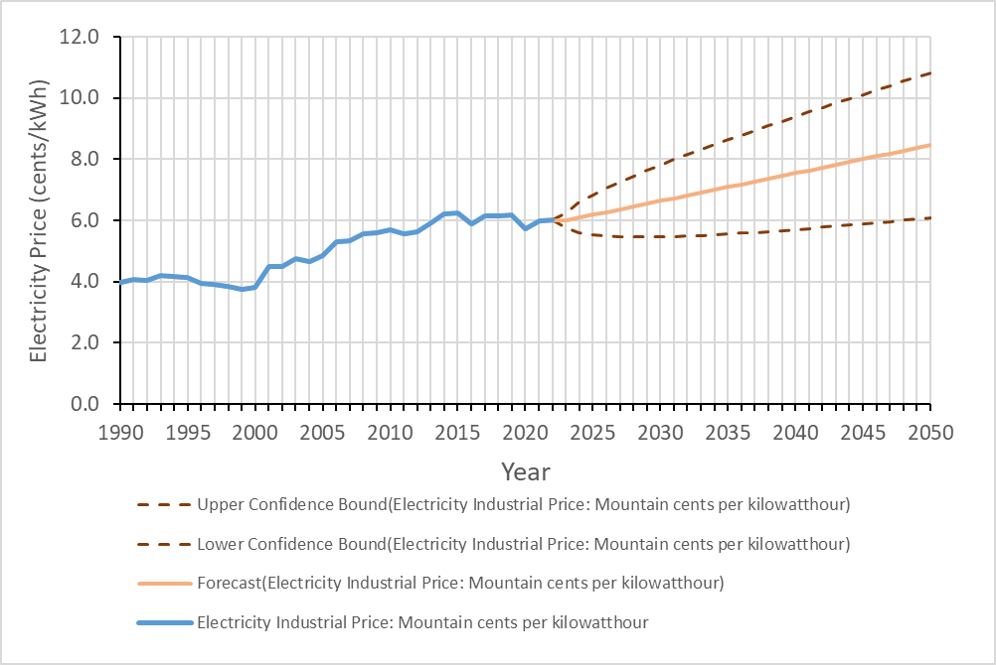
\includegraphics[width=.8\textwidth]{templates/images/Figure-EIA_Electricity_Forecast.png}
\caption[Electricity price forecast]{Price of electricity from the EIA Short-Term Energy Outlook \protect\citep{eia_short-term_2021}, forecast out to 2050.}
\label{fig:electricity_pricing}
\end{figure}

\section{Probabilistic Cost Model}\label{ch4:cm_uncertainties}
The model described thus far takes a deterministic approach; parameter values are fixed to their most-likely values when performing the NPV calculation. A probabilistic approach replaces these static values with distributions and repeatedly samples from those distributions to capture an ensemble of results. This Monte Carlo-style simulation can provide a more realistic assessment of system performance. However, all variables in the model have some underlying uncertainty, and defining distributions for every variable would add significant complexity to the model with diminishing returns. Variable selection can be performed using sensitivity testing to target the most impactful variables for uncertainty characterization. This helps balance model complexity with representativeness of the physical system. 

Recognizing the full probable range of variable values and the scenarios that trigger them requires a deep understanding of the scientific, engineering, and socio-technical elements influencing a system. For geothermal, subsurface characterization uncertainties play an important role, but so do uncertainties tied to public policy and market dynamics. The limited focus on the issues listed below should be considered fit-for-purpose for this thesis. Further analysis and discussion with subject matter experts on the local, state, and national levels is advised for similar analysis applied to an active geothermal project.

\subsection{Model Uncertainties}\label{ch4:model_uncertainties}
\subsubsection{Carbon Taxation}\label{ch4:carbon_tax_uncertainty}
\begin{wrapfigure}{R}{0.5\linewidth}
\centering
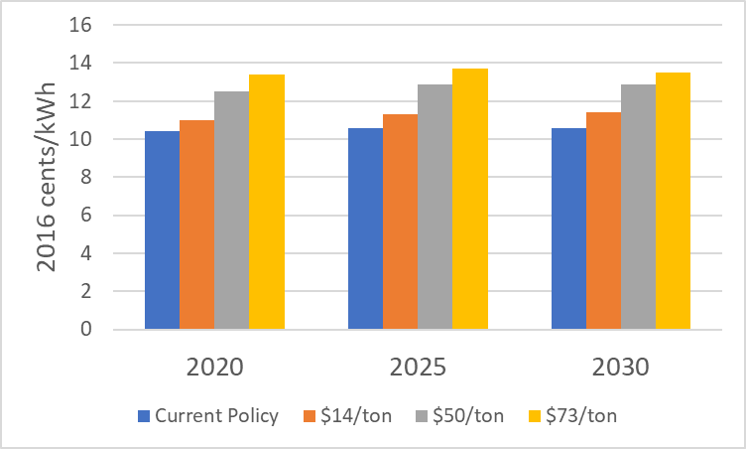
\includegraphics[scale=0.6]{templates/images/Figure-Carbon_Tax_Price_Impact.png}
\singlespacing
\caption[Carbon tax price impact]{National average retail electricity price changes with benchmark levels of carbon taxation, after \protect\citep[Figure\ 30]{larson_energy_2018}.}
\label{fig:carbon_tax_pricing}
\end{wrapfigure}
One proposal for advancing the transition to more renewable and sustainable energy solutions involves a carbon tax levied on fossil fuels. The SIPA Center on Global Energy Policy at Columbia University recently studied three analytical scenarios based on federal agency benchmark taxation rates of \$14/ton, \$50/ton, and \$73/ton CO$_2$-equivalent with annual percentage rate increases of 3, 2, and 1.5\%, respectively \citep{larson_energy_2018} (Figure \ref{fig:carbon_tax_pricing}). Their analysis forecasts the impact on electricity pricing out to 2030, with relatively steady-state implications that depend on the specified carbon tax rate. In all taxation cases, electricity prices increase over the present-day, no-tax scenario, likewise boosting the value of a zero-emissions geothermal power relative to fossil fuel-based options. The selected value range for sensitivity testing was a 0-28\% increase in wholesale price, which matches Figure \ref{fig:carbon_tax_pricing}.

\subsubsection{Future Electrification}\label{ch4:electrification_uncertainty}
NREL published a report earlier this year outlining the impact of heightened public trends away from non-electric sources of consumed energy, otherwise known as widespread electrification \citep{murphy_electrification_2021}. Some key findings include: (i) end-use natural gas consumption decreases, but so do natural gas prices, which can lead to an increase in natural gas-fueled power plants if no curtailments are imposed by fossil fuel policies, (ii) deployment of renewables will intensify overall, and (iii) local resources, potentially including new renewable power generation facilities, will mitigate the need for long-distance electricity transmission \citep{murphy_electrification_2021}.

\begin{wrapfigure}{R}{0.6\linewidth}
\centering
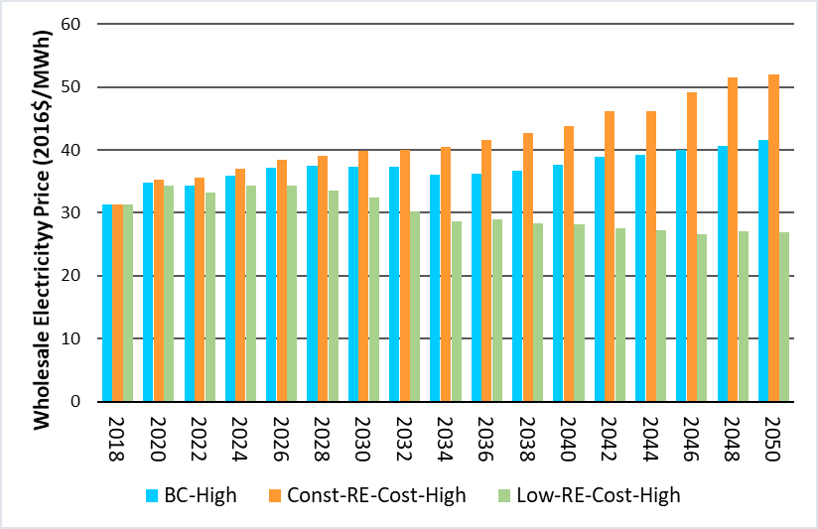
\includegraphics[scale=0.65]{templates/images/Figure-EFS_SIPA_Results.png}
\singlespacing
\caption[Electrification price impact]{Wholesale electricity price forecasts for high future electrification scenarios: base case (blue), constant renewable technology cost (orange), and low renewable technology cost (green). Cases are from the NREL Electrification Futures Study \protect\citep{murphy_electrification_2021}. Figure is adapted from interactive plots at \url{https://cambium.nrel.gov/? project=fc00a185-f280-47d5-a610-2f892c296e51.}}
\label{fig:EFS_electricification}
\end{wrapfigure}
The issue of national electrification is quite complex, particularly in predicting the interplay between the natural gas market and renewables. Additional dependencies include infrastructure upgrades and development to handle growing capacity, as well as local effects (e.g., permitting, water or electrical transmission, community support) that act as enablers or hurdles to building a new renewable-fueled power plant or expanding on existing power facilities. One way to simplify a model representation of widespread electrification is to incorporate swings in electricity prices similar to the scenarios shown in Figure \ref{fig:EFS_electricification} with the caveat that other related factors (e.g., federal and state-level incentive programs or infrastructure improvements) can also influence the bottom line for a geothermal project. Based on NREL projections for High Future Electrification cases, wholesale electricity prices in 2050 could vary from 23\% lower than baseline for the Low Renewable Technology Costs case to 50\% greater for the Constant Renewable Technology Costs case (Figure \ref{fig:EFS_electricification}). Therefore, -23\% and +50\% define the range of price factors used for sensitivity testing.
\\
\\
\subsubsection{Climate Change}\label{ch4:climate_uncertainty}
\begin{wraptable}{R}{0.58\linewidth}
\centering
\begin{tabular}{|l|c|c|}
\hline
\multicolumn{1}{|c|}{\textbf{Region}} & \textbf{RCP4.5} & \textbf{RCP8.5} \\ \hline
Northeast & 3.98 & 5.09 \\ \hline
Southeast & 3.40 & 4.30 \\ \hline
Midwest & 4.21 & 5.29 \\ \hline
Great Plains North & 4.05 & 5.10 \\ \hline
Great Plains South & 3.62 & 4.61 \\ \hline
\textbf{Southwest} & 3.72 & 4.80 \\ \hline
Northwest & 3.66 & 4.67 \\ \hline
\end{tabular}
\caption[Projected regional temperature changes]{Projected average temperatures in $^\circ$F for mid-century (2036-2065) relative to the 1976-2005 average baseline under lower emissions (RCP4.5) and higher emissions (RCP8.5) scenarios, adapted from \protect\citep[Table 6.4]{vose_temperature_2017}. New Mexico is included in he Southwest region, highlighted in bold.}
\label{tab:reg_climate}
\end{wraptable}

The $1.5^\circ$C climate change goal described in the 2018 IPCC special report \citep{ipcc_global_2018} refers to a global average, so more extreme temperature changes are expected to occur on a local scale even if this target gets met. New Mexico, a state already known for semi-arid conditions, is at risk of encountering warming far in excess of $1.5^\circ$C by 2050 (Table \ref{tab:reg_climate}). The North Carolina Institute for Climate Studies (NCICS) reports annual average temperatures in NM have already increased $1.1^\circ$C since the 1970s, and the observed number of days with maximum temperatures of $100^\circ$F ($37.8^\circ$C) or higher is rapidly climbing \citep{frankson_new_2019}.

Geothermal plant performance is sensitive to the temperature difference between the hot and cooled states of the working fluid. For air-cooled binary plants, changes in ambient temperature could impact overall power plant generation potential. In fact, geothermal power output typically shows seasonality, sometimes with variances of several percentage points in thermodynamic efficiency between winter and summer \citep[p.\ 52]{glassley_geothermal_2015}.  

\citeauthor{frankson_new_2019} present a range of model scenarios for temperature changes in New Mexico related to climate change (\citeyear[Figure 1]{frankson_new_2019}). The high emissions case predicts an average of $\approx 2.7^\circ$C and a maximum of $\approx 4.2^\circ$C increase in state-wide temperatures by 2050. An adjustment of 0-4.2$^\circ$C is therefore applied to this variable for cost model sensitivity testing.

\subsubsection{Drilling Costs}\label{ch4:drilling_uncertainty}
Studies consistently show drilling-related costs are the primary contributor to overall geothermal project expenses --- up to 60-75\% of the total cost of an EGS project \citep{lukawski_uncertainty_2016}. According to annual benchmark standards published by \citet{nrel_2020_2020}, future advances in geothermal drilling technology must address several factors for cost-reduction, including but not limited to: efficiencies in penetration rate and bit life, number of casing intervals, and consumption of drilling materials. All aspects of stimulation also must show improved economics to drive down costs \citep{nrel_2020_2020}.

Multiple scenario-based drilling cost curves were derived in association with the 2017 GeoVision study as potential updates for the GETEM model (Figure \ref{fig:drill_cost_curves}) \citep{lowry_implications_2017}. The following list covers the geothermal drilling technology advancements required to justify these curves \citep{augustine_geovision_2019}:
\begin{itemize}[itemsep=2pt]
    \item Bit life and rate of penetration scale from 2-4$\times$ faster than the base case.
    \item Number of casing intervals incrementally reduces to just one for the ideal case.
    \item Mud costs decline as greater fractions of the well use air drilling techniques.
    \item Logging while drilling (LWD) replaces wireline drilling for up to the entire well length in the ideal case.
    \item Contingency costs related to unexpected or adverse conditions drop from 15\% to 0\% across the four cases.
\end{itemize}

\begin{figure}
\centering
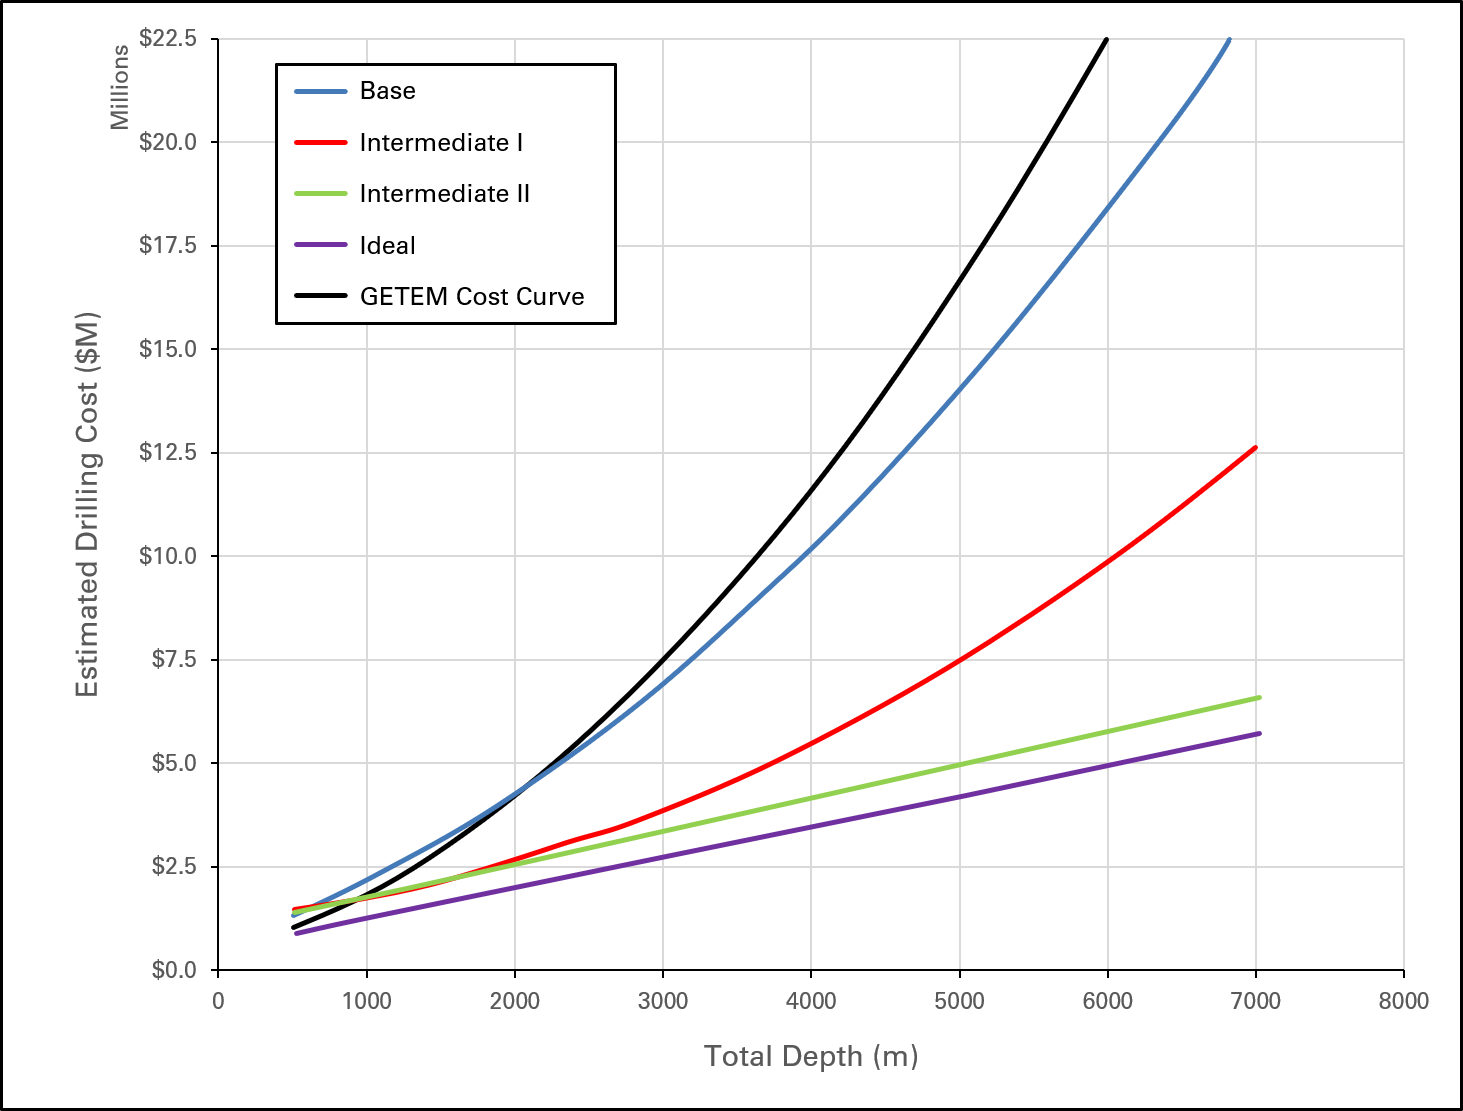
\includegraphics[width=0.8\textwidth]{templates/images/Figure-Drilling_Cost_Curves.png}
\singlespacing
\caption[GeoVision drilling cost curves]{Drilling cost curves in \$M USD per meters depth for a large-diameter open-hole vertical well, adapted from \citep[Figure 8]{augustine_geovision_2019}}
\label{fig:drill_cost_curves}
\end{figure}

In consideration of the cost curves in Figure \ref{fig:drill_cost_curves} and the anticipated depths for the target reservoir in the Lighting Dock expansion, the selected range of drilling costs to test for model sensitivity is \$1--\$3 million.

\subsubsection{Thermal Drawdown Rate}\label{ch4:drawdown_uncertainty}
Much like wells for water access or oil \& gas production, geothermal wells create drawdown effects from extended operations. The thermal drawdown rate defines how quickly the heat content (enthalpy) accessible within the reservoir fracture network declines over time. As thermal drawdown increases, the temperature of produced fluids decreases, as does the amount of electricity generated by the binary cycle process.

Recent EGS studies suggest 0.5--0.6\%/year is an appropriate drawdown rate for EGS \citep{augustine_geovision_2019}, although more pessimistic assessments range from 1.5\%/year \citep{beckers_low-temperature_2016}, to 3.3\%/year \citep{augustine_comparison_2006} and 4\%/year \citep{tester_economic_1990}. End-cap values of 0.5\% and 4\% are used for sensitivity analysis.

\subsubsection{Geothermal Gradient}\label{ch4:gradient_uncertainty}
As a blind geothermal system with no original surface expression, the Lightning Dock discovery only occurred after anomalously high temperature gradients (and boiling water) were found in local agricultural wells \citep{crowell_history_2014}. Table \ref{tab:ld_gradient_holes} lists bottom hole temperatures for wells drilled within a 0.5--4.0 km distance from the field-central TFD55-7 well during the 2001--2004 Geothermal Resource Evaluation and Definition (GRED) program \citep{cunniff_final_2005}. Note that the Gradient column in the table describes a linear fit from an assumed surface temperature of 15$^\circ$C to BHT, potentially over-simplifying complex temperature relationships with depth. The gradients in the Reported column come from more reliable assessments near well total depth (TD) as documented by \citet{cunniff_final_2003}. 
\\
\begin{table}%[!htp]
\centering
\begin{tabular}{|l|c|c|c|c|}
\hline
\textbf{Well Name} & \textbf{Depth (m)} & \textbf{BHT ($^\circ$C)} &
\textbf{\begin{tabular}[c]{@{}c@{}}Gradient\\(K/km)\end{tabular}} &
\textbf{\begin{tabular}[c]{@{}c@{}}Reported\\(K/km)\end{tabular}} \\ \hline
\textbf{TG12-7} & 305 & 69 & 177 & 120 \\ \hline
\textbf{TG56-14} & 381 & 36 & 55 & 80 \\ \hline
\textbf{TG36-7} & 305 & 90 & 246 & - \\ \hline
\textbf{TG57-7} & 278 & 108 & 335 & - \\ \hline
\textbf{TG52-7} & 771 & 137 & 158 & - \\ \hline
\end{tabular}
\caption[Lightning Dock well data]{Examples of Lightning Dock geothermal gradients from bottom hole temperatures (BHT). Gradient is a linear approximation assuming 15$^\circ$C at the surface. The two Reported gradients use temperature log trends near TD. Table adapted from \protect\citep[Table\ 1,][]{cunniff_final_2005}.}
\label{tab:ld_gradient_holes}
\end{table}

Thermal models calibrated to these wells show local gradients in excess of 300 K/km near the field center, and temperature inversions occur on the flanks of the main Lightning Dock thermal anomaly \citep[see Figs.\ 23--24,][]{cunniff_final_2005}. Away from this fault-centered hydrothermal plume --- where an EGS expansion project would be targeted --- the thermal field settles into a more traditional monotonically-increasing depth trend. Wells TG12-7 and TG56-14, located 1 km and 4 km away from TFD55-7, respectively, have reported gradients of 80--120 K/km. This range is used for testing model sensitivity to thermal gradient variations.

\subsection{Sensitivity Testing}\label{ch4:sensitivity}
Selecting which of the uncertainties discussed in Section \ref{ch4:cm_uncertainties} should be treated as probabilistic values in the cost model requires testing the sensitivity of NPV to model adjustments bounded by parameter uncertainty ranges. Specifically, NPV is recalculated after changing a single model variable at a time to match the extremal values outlined in the previous discussion. The full NPV calculation follows the model descriptions given in Sections \ref{ch4:cm_npv}--\ref{ch4:cm_params}, with the exception of price-related uncertainties, which are modeled by changing the price annually to mimic the most price-sensitive scenario where PPAs are market-based rather than fixed. No flexibility is assumed for this exercise, so the full power plant expansion takes place at the start of the 30-year timeline. Also, the sensitivity analysis uses the version of the static model where production flow rate is fixed at 40 kg/s (see Table \ref{tab:cm_resource_params}) and the capacity per module depends only on the temperature of the produced brine. The reasons for this choice of model structure over one where power output is strictly capped at 5 MW are discussed further in Chapter \ref{ch6:cm_results}.

The tornado diagram in Figure \ref{fig:tornado} provides a simple visualization of model sensitivity based on NPV calculation results for the different uncertainties, sorted in order of descending importance. Results also appear in Table \ref{tab:tornado_table}. The baseline static model predicts a NPV of $\approx \$91,000$. Results deviate from baseline most significantly for thermal drawdown rate; when no measurable drawdown takes place, NPV reaches \$18 million, but predicted losses top \$47 million if the drawdown rate is as high as 4\%. Uncertainties related to drilling costs, future electrification, and the geothermal gradient all show moderate importance for project NPV. Changes to ambient surface temperature (i.e., due to climate change) and pricing from carbon taxation both have an order of magnitude less influence on project NPV than other uncertainties. Based on this sensitivity test, variables tied to the top 4 uncertainties are treated as random variables for a probabilistic NPV model.

\begin{figure}%[!htp]
\centering
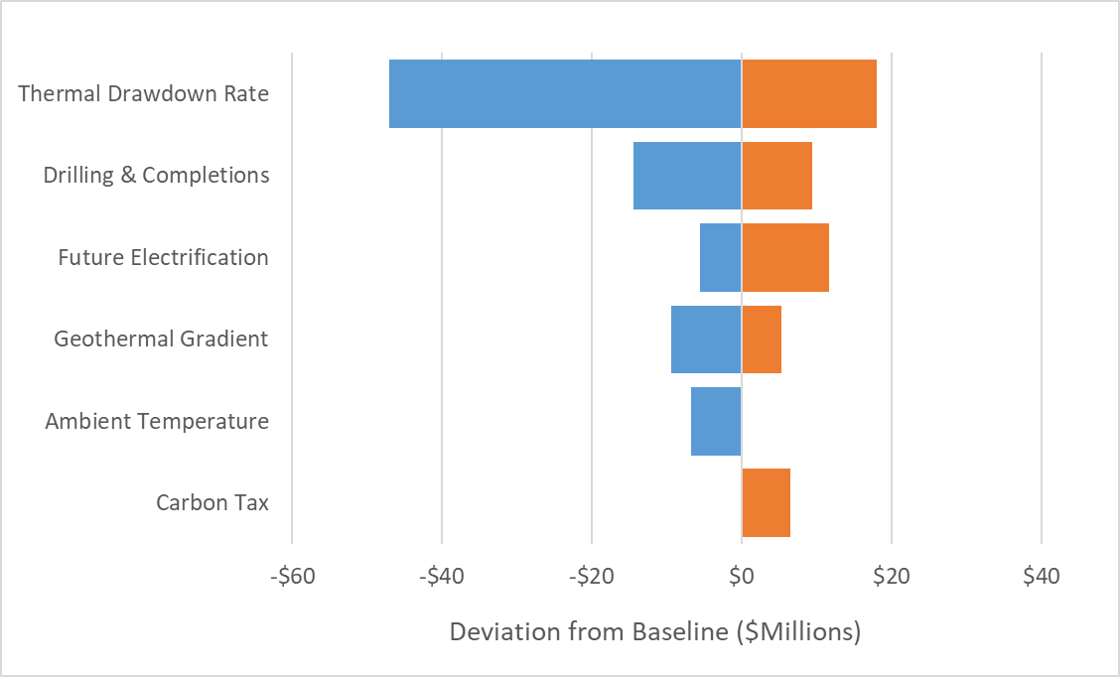
\includegraphics[width=0.8\textwidth]{templates/images/Figure-Tornado.png}
\singlespacing
\caption[Sensitivity testing tornado diagram]{Tornado diagram showing NPV model sensitivity to different system uncertainties for the proposed Lightning Dock expansion. X-axis measures deviation from base case when all plant construction takes place at project start and the model parameterization matches Tables \ref{tab:cm_resource_params}-\ref{tab:cm_econ_params}. Values are in \$M USD, where M indicates millions.}
\label{fig:tornado}
\end{figure}

\begin{table}%[!htp]
\centering
\begin{tabular}{|l|c|c|c|}
\hline
\textbf{} & \textbf{Low (\$M)} & \textbf{High (\$M)} & \textbf{Range (\$M)} \\ \hline
\textbf{Thermal Drawdown Rate} & -\$47.0 & \$18.0 & \$65.0 \\ \hline
\textbf{Drilling Costs} & -\$14.5 & \$9.4 & \$23.9 \\ \hline
\textbf{Future Electrification} & -\$5.5 & \$11.7 & \$17.2 \\ \hline
\textbf{Geothermal Gradient} & -\$9.4 & \$5.4 & \$14.7 \\ \hline
\textbf{Ambient Temperature} & -\$6.7 & -\$0.1 & \$6.6 \\ \hline
\textbf{Carbon Tax} & -\$0.1 & \$6.5 & \$6.6 \\ \hline
\end{tabular}
\caption[Sensitivity testing results]{Results of NPV model sensitivity testing for different system uncertainties associated with the Lightning Dock expansion. NPV values are listed in \$M USD, where M indicates millions.}
\label{tab:tornado_table}
\end{table}

\subsection{Probability Density Functions}\label{ch4:pdfs}
Having established the key uncertainties, \acrlong{pdf}s (\acrshort{pdf}s) can be assigned to the related model parameters for use as part of a stochastic NPV assessment. Running the model multiple times in succession creates a Monte Carlo ensemble of NPV solutions, each representing the model response to a different sampling of the parameter PDFs. The ensemble can be evaluated using a combination of metrics for individual model analysis or comparison with alternative models. Chapter \ref{ch6:cm_results} outlines the results of the Monte Carlo approach applied to the Lightning Dock expansion cost model using the PDFs in figure \ref{fig:cm_probdists} and described below.

\begin{figure}%[htp]
\centering
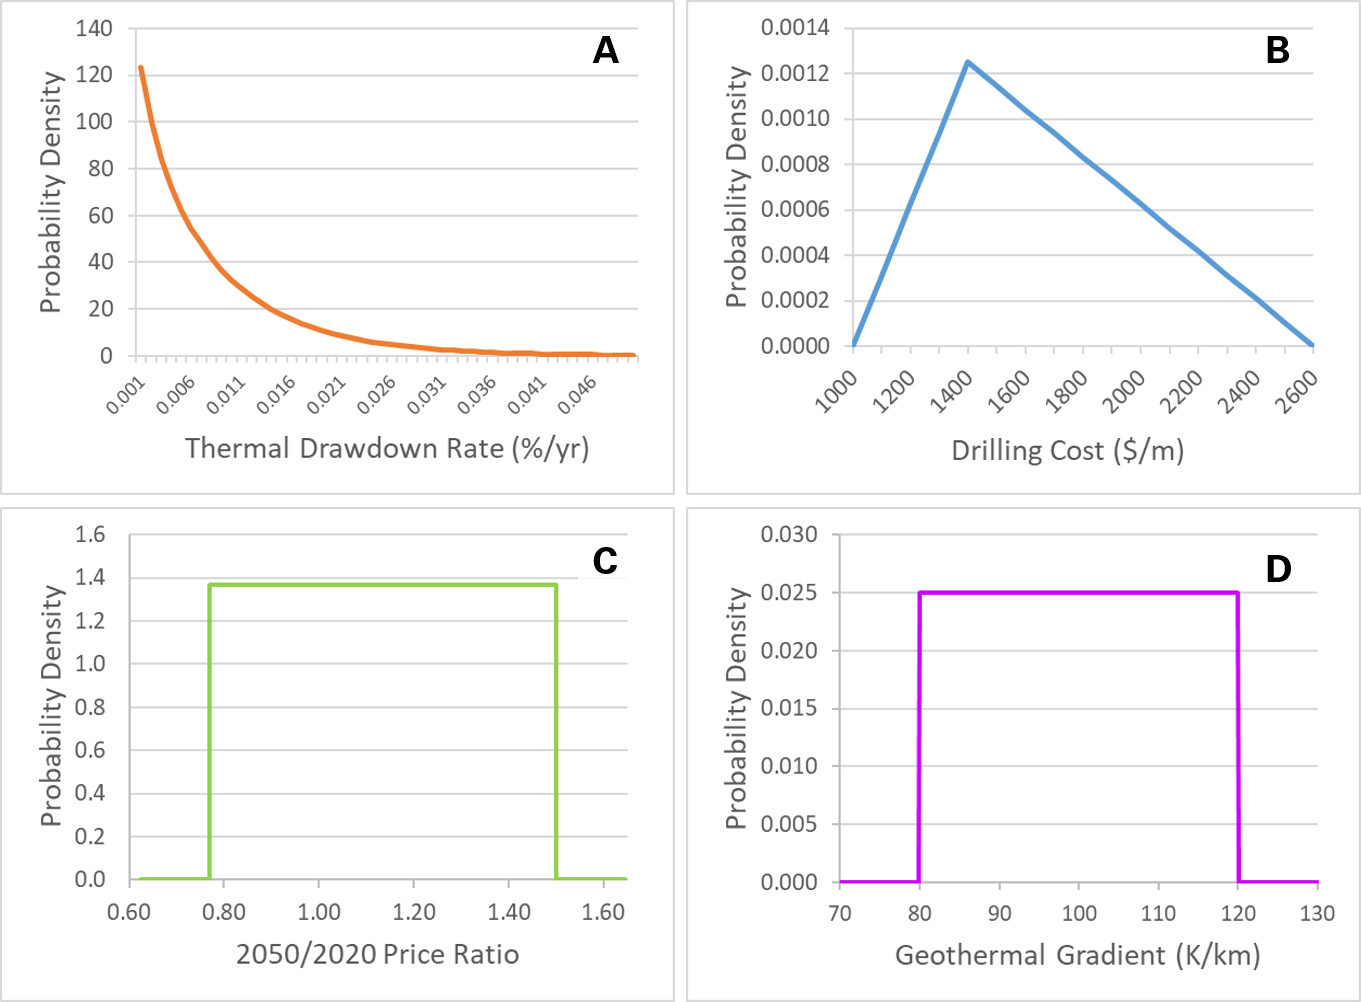
\includegraphics[width=.85\textwidth]{templates/images/Figure-ProbDists.png}
\singlespacing
\caption[Cost model probability distributions]{Probability distribution functions for A. thermal drawdown rate, B. drilling costs, C. electricity pricing, and D. geothermal gradient.}
\label{fig:cm_probdists}
\end{figure}

\subsubsection{Thermal Drawdown Rate}\label{cm4:prob_tdr}
The latest version of GETEM \citep{mines_getem_2016} and its variant in the NREL System Advisor Model \citep{blair_system_2018} apply 0.5\% as a default value for thermal drawdown rate. Higher decline rates tend to be associated with older references; 1-2\% for GEOPHIRES \citep{beckers_low-temperature_2016}, 3\% in a thesis by \citet{augustine_hydrothermal_2009}, and 4\% for work done in the 1990s by \citet{tester_economic_1990}. The probability density function for thermal drawdown was designed using a beta function such that the P$_{50}$ value aligns with 0.5\% annual drawdown rate, and 4.0\% represents the P$_{97.5}$ case (Figure \ref{fig:cm_probdists}A). Note that the beta function was slightly altered to follow a linear trend from P$_{95}$ to P$_{100}$ to ensure rare extremely high rates in the distribution function do not asymptotically approach over 10\% per year. The highest rate supported by the distribution is 5.6\%.

\subsubsection{Drilling Costs}\label{cm4:prob_dc}
Drilling costs for geothermal wells remain a topic of debate due in part to the small number of direct analogs, particularly for EGS wells, and the documented differences with oil \& gas drilling operations. This discrepancy was noted in the 2006 MIT study on EGS, which promoted the use of a dedicated geothermal drilling cost index as a solution \citep{tester_future_2006}. Nevertheless, numerous and sometimes quite disparate relationships have appeared in the years since; for the 1.0-1.5 km drilling depths considered in this study, recent estimates range from a low $\approx\$500$/m \citep{lukawski_uncertainty_2016} to a very high \$2,800/m \citep{lowry_implications_2017}. In order to capture a reasonable spread while recognizing the uncertainty in even defining a distribution shape, geothermal drilling costs are modeled as a triangular distribution (Figure \ref{fig:cm_probdists}B). The midpoint value of \$1400/m comes from the predicted well depth and cost in the static model (see Section \ref{ch4:cm_capex_dc}). The extreme values of \$1000/km and \$2800/km approximate the range shown for depths of 1.0--1.5 km among the drilling cost curves from the recent GeoVision study (Figure \ref{fig:drill_cost_curves}).

\subsubsection{Electricity Pricing}\label{cm4:prob_price}
Electricity prices in the static cost model are determined by the EIA STEO price forecast for the Mountain region (Figure \ref{fig:electricity_pricing}) \citep{eia_short-term_2021}. Two variable price components are superimposed on this trend for the probabilistic model. First, a disruption to the cost curve is simulated by randomly-selecting a year between 2020--2050 and introducing a step-change in price to capture the sudden nature of energy transition events. The magnitude of the step change is determined from a uniform distribution bounded by the range of 2050 High Future Electrification prices relative to the 2020 HFE base case in the Electrification Futures Study (Figure \ref{fig:cm_probdists}C) \citep{murphy_electrification_2021}. An example of how this randomly-timed, randomly-sampled step change affects the price curve is shown in Figure \ref{fig:elec_price_prob}A. 

Second, volatility could also influence the spot price used for setting a power purchase agreement for a given model year. Using the 95\% confidence bounds on the price curve to derive standard deviation, each point in the forecast is replaced by a normal distribution and randomly sampled to produce different price model realizations (Figure \ref{fig:elec_price_prob}B). This curve will regenerate as a unique price projection for each Monte Carlo realization of the cost model.

\begin{figure}[htp]
\centering
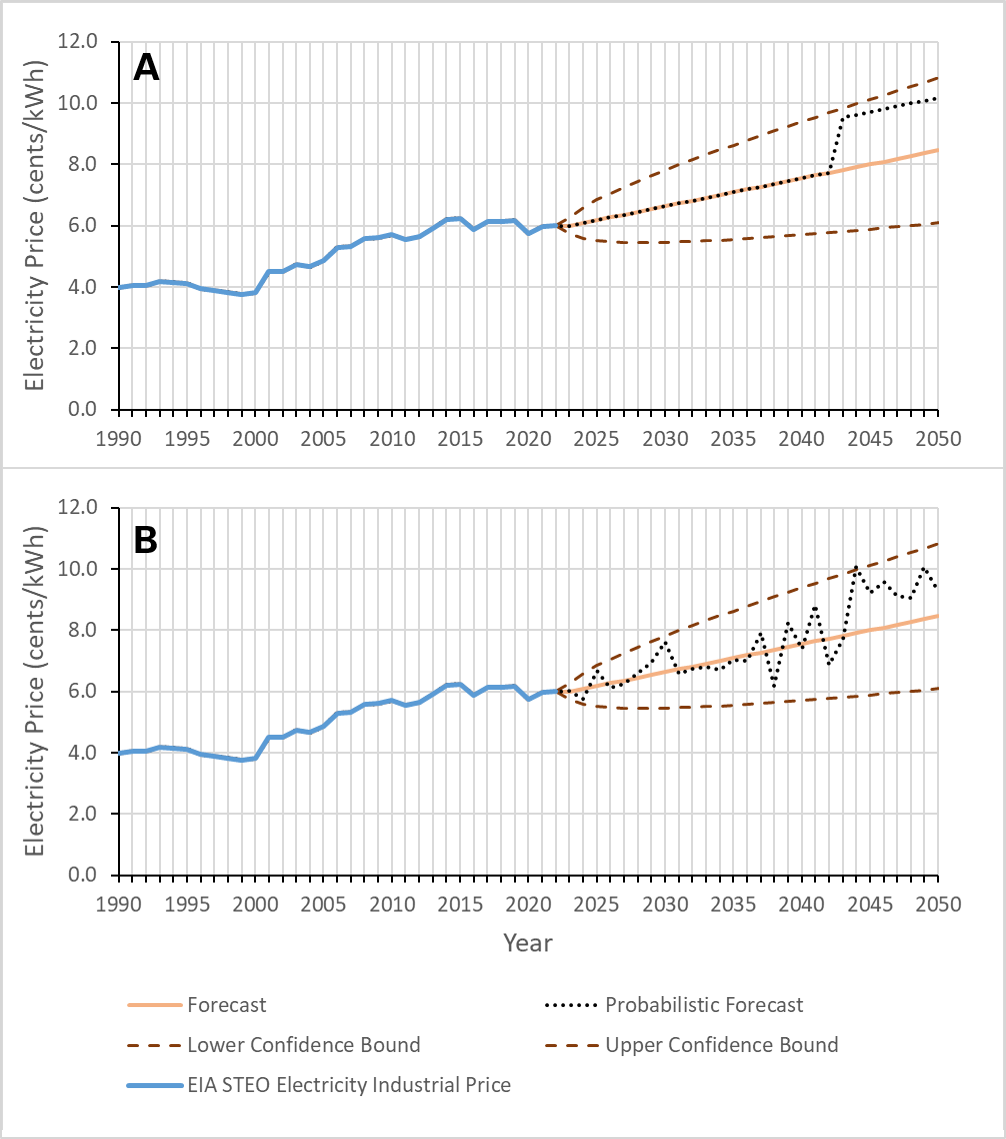
\includegraphics[width=.85\textwidth]{templates/images/Figure-ElectPrice_Prob.png}
\singlespacing
\caption[Cost model probabilistic price forecasts]{EIA STEO electricity industrial prices for the Mountain region (blue), forecast to 2050 (orange) as in Figure \ref{fig:electricity_pricing}, with A. a randomly-defined step change in pricing and B. added annual volatility using the forecast 95\% confidence intervals.}
\label{fig:elec_price_prob}
\end{figure}

\subsubsection{Geothermal Gradient}\label{cm4:prob_gradient}
Local spatial variations in geothermal gradient are difficult to characterize with only a sparse sampling of the Lightning Dock area by predominantly shallow boreholes. Subsurface models like those shown in Figures 22--24 of \citep{cunniff_final_2005} generally predict a smoothly-varying thermal field in areas without direct observational data. But the complex temperature structure associated with the Lightning Dock hydrothermal plume suggests thermal heterogeneity can exist away from the Animas Valley fault. Uncertainty in geothermal gradient is therefore represented in the cost model by a uniform probability distribution with end points determined by measured gradients from wells TG12-7 and TG56-14 (Figure \ref{fig:cm_probdists}D).

\subsubsection{Reservoir Temperature}\label{cm4:prob_temp}
Although not included in the sensitivity testing exercise in Section \ref{ch4:sensitivity}, the original proposal for EGS production at Lightning Dock by \citet{schochet_development_2001} noted a range of likely reservoir temperatures in the Horquilla limestone formation. Geothermal power production relies first and foremost on the subsurface temperatures being ``mined'' by circulating fluids. Uncertainty in initial reservoir temperature is therefore included in the cost model, represented by a uniform probability distribution with bounds determined from the temperatures proposed by \citet{schochet_development_2001} (Figure \ref{fig:cm_temp_pdf}).

\begin{figure}[H]
%\begin{wrapfigure}{R}{0.55\linewidth} %[htp]
\centering
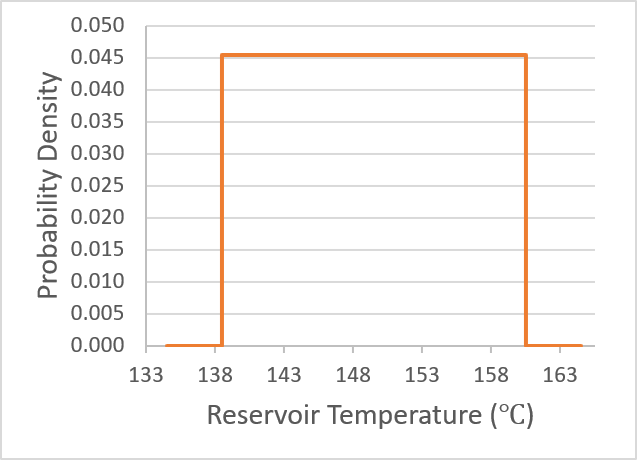
\includegraphics[scale=0.45]{templates/images/Figure-Reservoir_Temp_PDF.png}
\singlespacing
\caption[Reservoir temperature PDF]{Reservoir temperature probability density function. The value range is based on values originally proposed by \protect\citet{schochet_development_2001}.}
\label{fig:cm_temp_pdf}
%\end{wrapfigure}
\end{figure}

\section{Flexibility with Design Options}\label{ch4:flex_design_options}
The addition of probability density functions to the cost model for Monte Carlo simulation provides a means of testing the model response to uncertainties in the system. But this probabilistic Base Case model still remains inflexible in the face of emergent conditions that would trigger actions in a real-life scenario. These actions are sometimes characterized as design options that, like financial options, can be exercised in the future if doing so might benefit system stakeholders \citep[p.\ 270-272]{de_neufville_flexibility_2011}.

Design options define decision rules for how a model behaves based on past observations. Decision rules may act independently or be chained together to mimic complex system flexibilities that can reveal otherwise hidden financial value. The following scenarios extend the Base Case model with one or more decision rules. Chapter \ref{ch6:cm_results} examines how implementing these rules impacts predicted model ENPV, target curves, and other forecast performance measures described in Section \ref{ch6:cost_model_metrics}.

\subsection{Redevelop Only Case}\label{ch4:flex_redevelop_case}
Sensitivity testing revealed thermal drawdown rate as the most important uncertainty governing cost model performance (Figure \ref{fig:tornado}). Over time, cooling of the reservoir by injected fluids results in declining input temperatures to the binary cycle plant and hence lower electricity production. If the latter drops below a certain level, redrilling or restimulation of the reservoir are required to ensure generation rates remain within a reasonable (or profitable) range. The GETEM model tracks thermal decline and discounts power plant performance until the accessible reservoir temperature reaches a certain threshold defined by \citep{entingh_volume_2006}:
\begin{equation}
\label{eq:drawdown_threshold}
    \Delta T_{max} = (T_f-T_i)_{max} = 0.21 \cdot T_i - 12.2
\end{equation}

Combining this equation with a harmonic decline curve assumption results in the following relationship for the time before the maximum acceptable decline is reached:

\begin{equation}
\label{eq:redevelop_time}
\begin{aligned}
    t &= \frac{1}{D} \cdot 
    \left( {
    \left( {\frac{T_i}{T_f} }\right) - 1
    }\right)\\
    &= \frac{1}{D} \cdot 
    \left( {
    \left( {\frac{T_i}{1.21 \cdot T_i - 12.2}
    }\right) - 1
    }\right) 
\end{aligned}
\end{equation}

To counteract the negative impact of this decline, a full field re-drill campaign is triggered in cost models like GETEM. This may occur several times over the lifespan of a geothermal power plant depending on the drawdown rate, although GETEM freezes re-drills in the final 5 years to ensure no redevelopment cost is incurred just prior to end of life for the facility \citep{entingh_volume_2006}. This methodology is applied here using the following decision rule:
\\
\\
\textbf{Redevelopment Decision Rule}\label{ch4:dr_redevelop}
\begin{enumerate}
	\item Determine the temperature threshold for viable power production using Equation \ref{eq:drawdown_threshold} and the initial reservoir temperature.
	\item Calculate the number of years until the temperature threshold is reached based on the thermal drawdown rate and Equation \ref{eq:redevelop_time}. This defines the redevelopment interval for the field.
    \item In the annual cash flow analysis, determine if time since installation of any power plant modules is a multiple of the redevelopment interval. If so and the year being evaluated does not fall within the final 5 years of the project lifespan:
	\begin{enumerate}
	    \item Identify how many modules need to be redeveloped. Multiply this by 2 to define the number of wells being sidetracked (or redrilled). This assumes the wells are in pairs for each module.
	    \item Calculate CAPEX for redevelopment by multiplying the drilling costs per well by the number of wells being reworked, then discount by the pre-determined redevelopment factor. Scale this by the learning rate discount based on the number of wells already drilled since field operations began.
	    \item Update the running tally of wells drilled or redrilled to include wells from this redevelopment effort.
	    \item Reset the produced brine temperature to the initial reservoir temperature.
    \end{enumerate}
\end{enumerate}

\subsection{Redevelop \& Grow Case}\label{ch4:flex_grow_case}
Redevelopment of the geothermal field is primarily a mitigation against loss of accessible resource as thermal drawdown impacts the flow paths between wells. Capturing upside potential is equally important. The Redevelop \& Grow case recognizes that up-swings in wholesale electricity prices may signal a comprehensive shift in long-term energy pricing due to influences like societal shifts toward electrification. To take advantage of the opportunity, this case considers a price change threshold (\textit{Price trigger for flexibility}, see Table \ref{tab:cm_econ_params}) as the trigger for installing additional geothermal power plant modules and renegotiating the PPA with the local utility company. The scenario assumes a flat percentage increase in capacity (\textit{Expansion amount}, see Table \ref{tab:cm_econ_params}) and universal success in establishing new power agreements at a set mark-up percentage above wholesale (\textit{Contract rate over wholesale}, see Table \ref{tab:cm_econ_params}). The field redevelopment decision rule outlined for the Redevelop Only case remains intact, and another decision rule for design flexibility in modular growth is as follows:
\\
\\
\textbf{Capacity Growth Decision Rule}\label{ch4:dr_grow}
\begin{enumerate}
    \item In the annual cash flow analysis, look up the predicted wholesale electricity price for the current year and determine the deviance between this price and the wholesale price used in the last PPA contract (i.e., when the last capacity change took place). Here, deviance is defined as: \(\frac{(\text{current price} - \text{past price})}{\text{past price}}\).
    \item If the deviance exceeds the pre-set price trigger and the year being evaluated does not fall within the final 5 years of the project lifespan:
    \begin{enumerate}
        \item Multiply the number of operating power plant modules in the field by the pre-set expansion parameter to determine the number of modules to add.
        \item Calculate CAPEX for drilling an injector-producer pair for each added module. Scale this value by the learning rate discount based on the number of wells previously drilled or redrilled in the field.
        \item Update the tallies for the number of modules in the field and the number of wells drilled or redrilled to include the added modules and their wells.
        \item Determine the new PPA contract price by multiplying the predicted wholesale electricity price for the current year by the pre-determined contract rate above wholesale factor.
    \end{enumerate}
\end{enumerate}

\subsection{Full Flexibility Case}\label{ch4:flex_reduce_case}
Price swings can go the opposite direction as well. The NREL Electrification Futures Study \citep{murphy_electrification_2021} identified scenarios where electricity prices fall between 2020 and 2050, so having a means of addressing a future with tighter margins would be a useful flexibility. In the Full Flexibility Case, field redevelopment with thermal degradation and capacity increases in response to price surges remain in effect. In addition, a sudden drop in electricity prices (\textit{Price trigger for flexibility}, see Table \ref{tab:cm_econ_params}) serves as a trigger for the power plant operator to remove or decommission a number of binary cycle modules (\textit{Reduction amount}, see Table \ref{tab:cm_econ_params}). Since modules operate independently with their own injector-producer couplet, they can be individually decommissioned with no impact on other installed modules in the aggregate facility. Additional cost savings might be realized if the modules are leased and equipment can be returned early to the vendor when no longer in use, although for the sake of simplicity, this option has not been included in the cost model. The decision rule for price-based decommissioning of active modules is as follows:
\\
\\
\textbf{Capacity Reduction Decision Rule}\label{ch4:dr_reduce}
\begin{enumerate}
    \item In the annual cash flow analysis, look up the predicted wholesale electricity price for the current year and determine the deviance between this price and the wholesale price used in the last PPA contract (i.e., when the last capacity change took place). Here, deviance is defined as: \(\frac{(\text{current price} - \text{past price})}{\text{past price}}\).
    \item If the deviance is negative and exceeds the pre-set price trigger (in magnitude), and the current year does not fall within the final 5 years of the project lifespan:
    \begin{enumerate}
        \item Multiply the number of operating power plant modules in the field by the pre-set reduction amount parameter to determine the number of modules to decommission.
        \item Reduce the count of operating modules in the field to account for taking these modules offline.
        \item Make sure OPEX is only calculated for operating power plant modules.
        \item Do \underline{not} reduce the running tally of wells drilled or redrilled. Shutting down modules does not negate the learning experience of drilling the wells associated with those modules.
    \end{enumerate}
\end{enumerate}

\section{Recap} \label{ch4:recap}
This chapter covered the methodology for using cost models to mitigate the risk of expanding an existing power facility with geothermal production. The Lightning Dock KGRA and present-day power plant are the subject of a hypothetical 5 MW EGS expansion project. The model assumes a 30-year useful life for the expansion, and construction is based on the deployment of pre-fabricated binary cycle modules with one injector-producer pair per module.
\\
\\
The modeling strategy follows a step-wise increase in model complexity:
\begin{enumerate}
    \item Start with a static model that calculates NPV based on estimates for Revenue, CAPEX, and OPEX. The model includes thermal drawdown of the reservoir, power plant degradation, a learning rate for drilling costs, and a discount rate for the time value of money. All parameters are pre-defined.
    \item Replace the static model with a probabilistic one by assigning probability density functions to key model parameters. Sensitivity testing high-grades which parameters to treat as uncertain in the model. Results are obtained through Monte Carlo sampling to build a solution ensemble, evaluated by multiple measures like ENPV, NPV percentiles, and target curves. Variables defined with PDFs in this analysis include: thermal drawdown rate, drilling costs, electricity pricing, geothermal gradient, and reservoir temperature.
    \item Incorporate flexibility with design options as decision rules in the probabilistic model. The decision rules being evaluated in this analysis include: field redevelopment due to thermal drawdown, growth in capacity when prices surge, and capacity reductions when prices decline.
\end{enumerate}

Results from applying these methods in the context of a risk-mitigation strategy for geothermal production are explored in Chapter \ref{ch6:cm_results}. 